%!TEX root = ../thesis.tex
%*******************************************************************************
%****************************** Fifth Chapter *********************************
%*******************************************************************************

\chapter{Population-scale differentiation of iPSCs to a neuronal fate}
\label{chapter5}

The study described in chapter 4 acted as a proof of principle study where we demonstrated that feasibility of pooling cells from several lines prior to differentiating.
This means that in a single experiment we can obtain data from multiple independent donors, thus allowing to perform population-scale studies.
The single cell readout allows to trace back the donor of origin of each cell, without the need of any barcoding.
We and other have shown that single cell RNA-seq can be used to map eQTL and despite the pooling we retain enough cells per individual to do so successfully.
Additionally, by profiling differentiations across several lines we can start to disentangle differences in differentiation efficiency across different lines and experimental batches.\\

In this second study, we scale up the study in terms of both donors (215 vs 125) and cells (over 1 million vs around 40,000) and apply similar principles to a much longer and more complex differentiation protocol, considering iPSCs differentiating towards a midbrain neuronal fate.\\

First, the use of the droplet-based scRNA-seq technology allows us to assay a much larger number of cells providing an overview of the plethora of brain cell types generated by this protocol. 
Moreover, the larger number of cell lines included and the longer protocol allows us to dive deeper into the differences across lines in efficiency to differentiate, and allows us to start exploring possible causes.
Finally, the closer resemblance of the differentiated cells to primary tissues allows to start looking into the effects of disease-associated variants onto specific cell types and across development. \\

Briefly, the dataset we describe in this chapter is genome-wide single cell RNA-sequencing profiling of over one million differentiating iPS cells collected from cell lines from 215 healthy donors. 
Data is collected at three maturation stages following differentiation to midbrain dopaminergic neurons: progenitor-like state (day 11), young neurons (day 30), and more mature neurons (day 52). 
Additionally, just before the latest time point half of the cells were stimulated with rotenone, to simulate oxidative stress. 

\newpage

\begin{Comment2}

\hspace{-3mm}\textbf{Contributions} This work is the result of a collaboration between the Stegle, Merkle, Marioni and Gaffney labs, and was funded by Open Targets 
(https://www.opentargets.org).
The data was generated by Dan Gaffney’s lab at the Wellcome Trust Sanger Institute, and the experiments were led by Julie Jerber, who also contributed to the interpretation of the results. 
The statistical methods and analyses described in this chapter were co-supervised by Dan Gaffney and Oliver Stegle. 
Daniel Seaton processed the data and performed \gls{qc}. 
Daniel and I developed and implemented the statistical methods under the supervision of Oliver Stegle and Dan Gaffney with some input from Florian Merkle, John Marioni and Natsuhiko Kumasaka.
In particular, Natsuhiko performed the colocalisation analysis.
The code for processing, analysing and plotting the data is open source and freely accessible here: https://github.com/single-cell-genetics/singlecell\_neuroseq\_paper.
Julie Jerber, Daniel Seaton, Florian Merkle, Dan Gaffney, Oliver Stegle and I wrote the manuscript, with input from Natsuhiko Kumasaka and John Marioni.
A preprint \cite{jerber2020population} can be found on biorxiv: https://www.biorxiv.org/content/10.1101/2020.05.21.103820v1, as:\\

Julie Jerber*, Daniel D. Seaton*, Anna S.E. Cuomo*, Natsuhiko Kumasaka, James Haldane, Juliette Steer, M Patel, D Pearce, M Andersson, Marc Jan Bonder, Ed Mountjoy, Maya Ghoussaini, Madeline A. Lancaster, the HipSci Consortium, John C. Marioni, Florian T. Merkle, Oliver Stegle, Daniel J. Gaffney. Population-scale single-cell RNA-seq profiling across dopaminergic neuron differentiation, 2020 (* equal contributions).

\end{Comment2}

\newpage

\section{Introduction}

As discussed, genetic variation can significantly alter cell function, for example by altering gene expression. 
Human iPSCs are a promising cellular model for assessing the cellular consequences of human genetic variation across different lineages, developmental states and cell types. 
In particular, human iPSCs facilitate the study of developmental time points and stimulation conditions that would be challenging to obtain \textit{in vivo}. 
The creation of cell banks containing hundreds of iPSC lines \cite{kilpinen2017common} provides an exciting opportunity to carry out population-scale studies \textit{in vitro} \cite{cuomo2020single, strober2019dynamic, schwartzentruber2018molecular, alasoo2018shared}.
However, differentiating iPSCs is expensive and labour-intensive, and differentiation experiments are difficult to compare due to substantial batch variation. 
Thus, studies of more than a handful of lines remain a significant challenge.
Furthermore, most iPSC differentiation protocols produce a heterogenous population of cells of which the target cell type is a subset \cite{d2019vitro, banovich2018impact, volpato2018reproducibility, nguyen2018single}. 
This variability in differentiation outcomes hinders efforts to dissect the genetic contributions to cellular phenotypes.\\

Single cell sequencing has enabled “multiplexed” experimental designs, where cells from multiple donors are pooled together \cite{cuomo2020single, nguyen2018single}. 
Pooling improves throughput and allows experimental variability between differentiation batches to be rigorously controlled, by enabling cell type heterogeneity to be accounted for in downstream analysis. 
To date, multiplexed experimental designs have only been applied to short differentiation protocols (over a period of days), that generate cells corresponding to very early stages of development, and have not captured developmental progression toward a mature cell fate. 
Population-scale pooling during long-term differentiation offers the opportunity to examine the effect of common genetic variants on gene expression in each cell population produced over neural development, providing a foundation for future mechanistic studies.\\

Here, we develop and apply a multiplexing strategy to profile the differentiation and maturation of more than two hundred iPSC lines derived from \gls{hipsci} towards a midbrain neural fate, including dopaminergic neurons (DA). 
DA are involved in motor function and other cognitive processes and play key roles in neurological disorders, including Parkinson’s Disease (PD)\footnote{Parkinson’s disease (PD) is a progressive neurodegenerative disorder, characterized by the loss of midbrain DA neurons. 
These neurons control motor behavior, and, as they degenerate, they result in several motor features of the disease, such as bradykinesia, rigidity, resting tremor, gait disturbances and postural instability \cite{lees2009parkinsons}.} \cite{osborn2017seq, stoddard2020stem}. 
To study how these cells differentiate, and how genetic background could influence differentiation, we employed a well-established protocol \cite{kriks2011dopamine} and collected cells at three maturation stages (progenitor-like, young neurons, and more mature neurons), covering 52 days of differentiation. 
We additionally exposed half of the cells on day 51 to rotenone, to explore how genetic variation shapes the neuronal response to oxidative stress. 
Using this system, we create the first map of \gls{eqtl} at multiple stages of human neuronal differentiation, and identify nearly 500 novel trait / \gls{eqtl} colocalisations. 
Using estimates of cell population composition based on single cell RNA-seq, we demonstrate that a strong, cell intrinsic-differentiation bias affects a significant proportion of \gls{ipsc} lines, such that approximately 25\% reproducibly fail to produce any neuronal cells.\\

% longer iPSC differentiation protocol

% relevant for cell therapy (dopaminergic neurons and PD)

% different 

\newpage

\section{Single cell map of iPSCs neuronal differentiation}

\subsection{Experimental strategy and data generation}

We selected 215 iPSC lines from 215 unique, healthy, unrelated donors from the \gls{hipsci} consortium.
Though in \gls{hipsci} multiple iPSC lines are available for the same donor, here we chose to maximise genetic heterogeneity and get lines all from different donors.\\

iPSC lines were cultured..

24h after plating, neuronal differentiation of the pooled lines to a midbrain lineage was performed as described by Kriks \textit{et al} \cite{kriks2011dopamine}.

The time points of collection (day 11, 30 and 52) were selected based on the data available in the original paper by Kriks \textit{et al}., \cite{kriks2011dopamine} where molecular profiling, biochemical and electro-physiological data defined developmental progression of midbrain DA neurons. 
In their paper they described days 11, 25, 50 and 80 as, respectively, midbrain DA progenitors, time of cell cycle exit, long term neurons and electro-physiologically active neurons. 
We therefore aligned our timeline with theirs and selected day 30 instead of day 25 to enrich for young post-mitotic neurons. 
% Analysis beyond day 52 were XXX

% Maybe briefly add what molecules are added and to mimick what.
% LDNSB, ..?

Day 11 should correspond to week 5 which is the beginning of neurogenesis \textit{in vivo}. 

Each pool contained cells from between 7 to 24 lines.

Droplet based scRNA-Seq was performed using the 10X Genomics™ technology \cite{zheng2017massively}.

\begin{figure}[h]
\centering
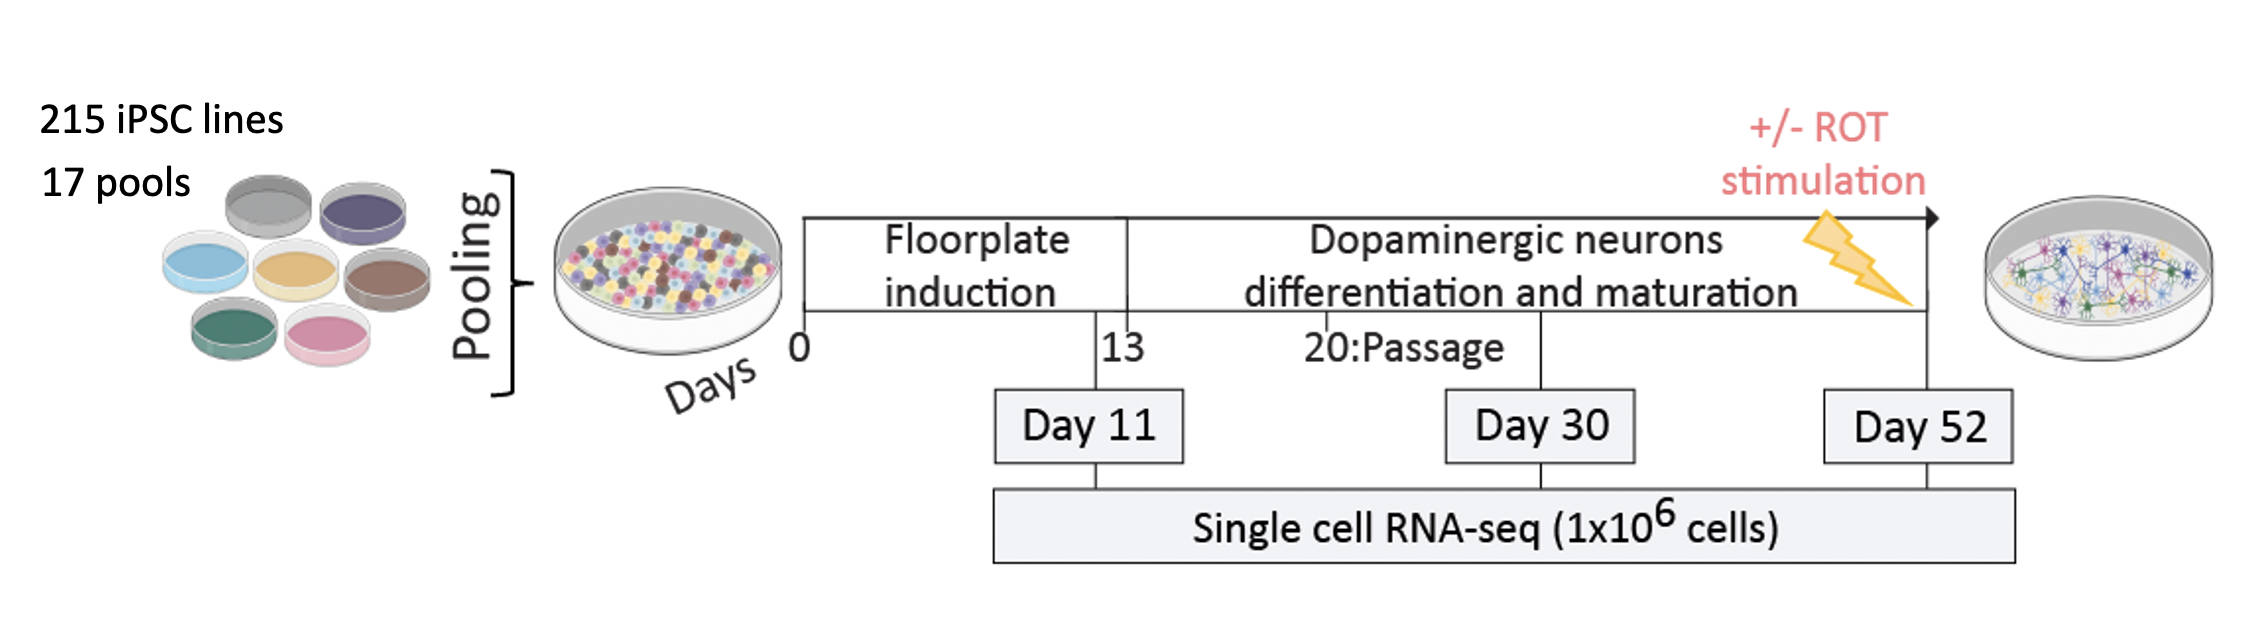
\includegraphics[width=16cm]{Chapter5/Fig/neuroseq_experimental_design.png}
\caption[Experimental Design]{\textbf{Experimental Design}.\\
Experimental design for pooled differentiations of iPSC to midbrain dopaminergic neurons. 
Time points at which cells were collected for scRNA-seq profiling (day 11, day 30, day 52) are indicated. 
On day 51, half of the cells were stimulated with rotenone (ROT) for 24h to induce oxidative stress.
Data from 215 iPSC lines (for 215 donors) across 19 pools were collected for a total of over a million cells.}
\label{fig:neuroseq_experimental_design}
\end{figure}

\subsection{Data processing and QC}

For each of 19 pooled experiments, donors (i.e. cell lines) were demultiplexed using demuxlet \cite{kang2018multiplexed}, using genotypes of common exonic variants (MAF > 1\%) available from the HipSci bank, and a doublet prior of 0.05. 
Only single cells with successful donor identification were retained for further analysis. 
This step filtered out two types of droplet: those containing two or more cells from different individuals, and those containing no cells, but that contained a mixture of free-floating RNA and had therefore passed the CellRanger UMI filter.

\section{Data overview}

We selected 215 iPSC lines derived from healthy donors by the HipSci project \cite{kilpinen2017common} for differentiation towards a midbrain cell fate, including dopaminergic neurons \cite{kriks2011dopamine}. 
Differentiation experiments were multiplexed using pools containing between 7 and 24 cell lines per experiment. 
Immunochemistry confirmed that cells from both pooled and conventional differentiation of individual lines expressed protein markers associated with patterning of DA (LMX1A, FOXA2 and TH). 
To capture transcriptional changes during neurogenesis and neuronal maturation, we performed single cell RNA sequencing (scRNA-seq) of cells captured at day 11 (day 11, midbrain floorplate progenitors), day 30 (day 30, young post-mitotic midbrain neurons) and day 52 (day 52, more mature midbrain neurons). 
To mimic an oxidative stress condition, we also profiled day 52 neurons upon exposure to a sub-lethal dose of rotenone (ROT, 0.1 μM; 24 h) a chemical stressor that preferentially leads to DA death in models of PD \cite{xiong2012mitochondrial}.

\subsection{Normalisation, dimensionality reduction, and clustering}

After QC, we obtained a total of 1,027,401 cells across 19 cell pools \cite{blondel2008fast} and four conditions. 
The cell line of origin for each cell was inferred from single cell RNA-seq read data using known genotypes made available by the HipSci consortium (using demuxlet, \cite{kang2018multiplexed}). 

Independent analysis of each time point allowed efficient batch effect correction (as all samples were from the same time point, containing similar mixtures of cell types), as well as reducing computational demands (by reducing the number of cells analysed together).
In particular, the following steps were performed: counts were normalised to the total number of counts per cell. 
Only genes with non-zero counts in at least 0.5\% of cells were retained. 
The top 3,000 most variable genes were then selected, after controlling for mean-variance dependence in expression data. 
The first 50 principal components (PCs) were calculated. 
Batch correction was applied on the level of PCs using Harmony \cite{korsunsky2019fast}, with each 10x sample treated as a distinct batch. 
UMAP and clustering was performed using these transformed PCs. 
Clustering was performed using Louvain clustering \cite{blondel2008fast} with 10 nearest neighbours. 
Analysis steps besides batch correction were carried out using the Scanpy package 58 \cite{wolf2018scanpy}. 

This identified a total of 26 clusters (6, 7 and 13 clusters respectively at day 11, day 30, day 52, Fig. \ref{fig:neuroseq_clusters}). 

\begin{figure}[h]
\centering
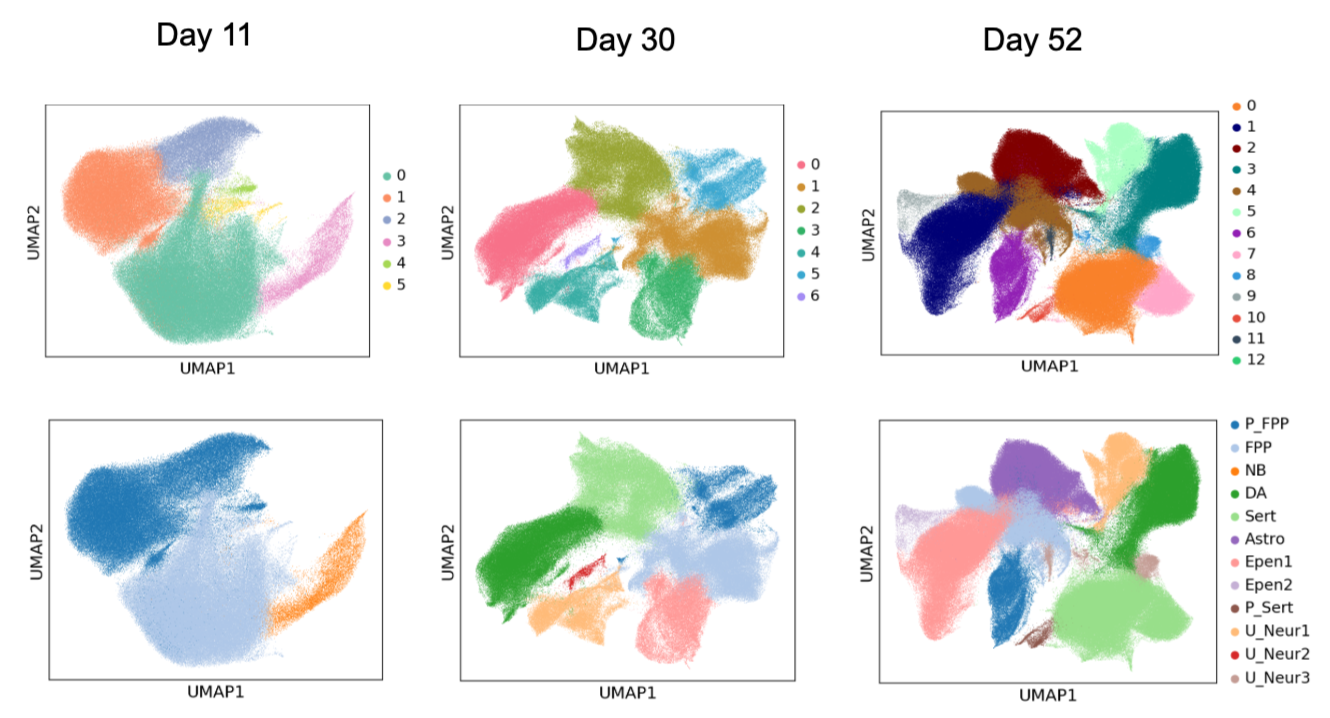
\includegraphics[width=16cm]{Chapter5/Fig/neuroseq_clusters_celltypes.png}
\caption[Clustering and cell type assignment]{\textbf{Clustering and cell type assignment}.\\
At each individual time point (day 11, day 30, day 52), cells were clustered using Louvain clustering, after normalization and batch correction using Harmony \cite{korsunsky2019fast}.
Subsequently, clusters were assigned to cell types using known marker genes. 
When two clusters showed the same gene set enrichment they were computationally assigned to the same cell type identity. 
(a) UMAPs of cells sampled at each time point and coloured by cell clusters. 
(b) UMAPs of cells sampled at each time point and coloured by assigned cell types.
Astro: Astrocyte-like, DA: Midbrain dopaminergic neurons, Epen1,Epen2: Ependymal-like, FPP: Floor Plate Progenitors, NB: Neuroblasts, P\_FPP: Proliferating Floor Plate Progenitors, P\_Sert: Proliferating serotonergic neurons, Sert: Serotonergic neurons, U\_Neur: Unknown Neurons.}
\label{fig:neuroseq_clusters}
\end{figure}

Clusters were mapped to cell types using a set of literature-curated 48 marker genes of major brain cell types. 
When two clusters show the same gene set enrichment they were assigned the same cell type identity
These clusters were then assigned to cell types by testing for enrichments of 48 literature-curated marker genes of major brain cell types.\\

\subsection{Cell type annotation}

% Among these, we identified six dominant cell types that were making up at least 10\% of the cells at any time point. 

\subsubsection{Day 11}

We identified two main cell type populations at day 11: proliferating and non-proliferating midbrain floorplate progenitors (both expressing \textit{LMX1A, FOXA2} and expressing \textit{MIK67, TOP2A} when proliferating \cite{la2016molecular}).
Together, these two made up around 96\% of cells at day 11.

We also identified a neuroblast (NB) population, (4\% of all cells at day 11) expressing pro-neuronal genes (\textit{NEUROD1, NEUROG2, NHLH1} \cite{bertrand2002proneural, lacomme2012neurog2})

\subsubsection{Day 30}

At day 30, we still had some floorplate progenitors (23\%) and proliferating progenitors (7\%), whereas the neuroblast population was not seen any longer.
Additionally, five new cell types were identified.
Four of these additional cell types appeared neuronal and one was non-neuronal (characterised by expression and lack of the pan-neuronal markers \textit{SNAP25} and \textit{SYT1} respectively). 

% \cite{arenas2015make}

The neuronal populations included two that could be assigned to a midbrain neuron identity, dopaminergic (DA, 27\%) and serotonergic (Sert, 21\%) neurons.
In particular, midbrain DA neurons expressed \textit{NR4A2, PBX1, TMCC3} \cite{la2016molecular, park2006acquisition, ramonet2012park9} whereas serotonergic neurons (Sert) expressed \textit{TPH1, TPH2, GATA2} \cite{cummings2019serotonergic}. 

One additional large neuronal population (expressing \textit{SNAP25} and \textit{SYT1}) expressed both midbrain DA markers and cortical marker, thus could not be assigned to a specific neuronal identity (Unknown neurons 1, around 8\%).
Finally, one more small neuronal population (less than 2\%) could also not be assigned to a specific identity (Unkown neurons 2). 

The non-neuronal cell type expressed all the classical markers of ependymal-like cells (Ependymal 1 \cite{campbell2017molecular}, 11\%). 

\subsubsection{Day 52}

At day 52 we largely recapitulated all of the same cell types identified at day 30.
Floorplate progenitors were present in smaller proportions (XX and YY \%).

In addition to DA, Sert, the unknow neuronal population 1 and the two ependymal cells we identified a population of astrocyte-like cells, which were unique to day 52 (Astrocyte-like \cite{sloan2017human, zhang2016purification}). 
Finally, we identified three additional rare cell types (<2\% of cells sampled at any time point), including a second ependymal-like population (Ependymal 2), a proliferating neuronal serotonergic population (Prolif. Serotonergic neurons), and one additional neuronal populations which could not be annotated unambiguously (Unknown neurons 3).

\begin{Abstract}
\textbf{Cell type notation}

DA: dopaminergic neurons;
Sert: serotonergic neurons;
FPP: floor plate progenitors;
P\_FPP: proliferating floor plate progenitors;
NB: neuroblasts;
Epen1: ependymal-like cells;
Astro: astrocyte-like cells
\end{Abstract}

\subsection{Overview}

For visualisation purposes, we also performed a combined analysis of a random subsample of 20\% of cells (after QC) from all time points.
In this case, the Harmony batch correction was performed across pools (rather than individual 10x sample).

A joint UMAP projection of cells collected across all time points, stimuli and lines revealed broad co-clustering of cell types, but with noticeable differences between time points and stimuli. 
We observed substantial variation in the cell type proportions across time points
and stimuli. 
For example, the proportion of DA upon ROT stimulation was significantly reduced (30\% reduction upon stimulation, Fisher’s exact test, p value=$2.2x10^{-16}$ ), consistent with previous observations that dopaminergic neurons are most affected by apoptosis due to oxidative stress \cite{sherer2003mechanism, knonagel1992autologous, cannon2009highly}.
Collectively, our population-scale scRNA-seq analysis revealed a diverse repertoire of cell types, enabling study of both cell line differentiation propensity and the identification of genetic variants that act in a cell type-specific manner.

\begin{figure}[h]
\centering
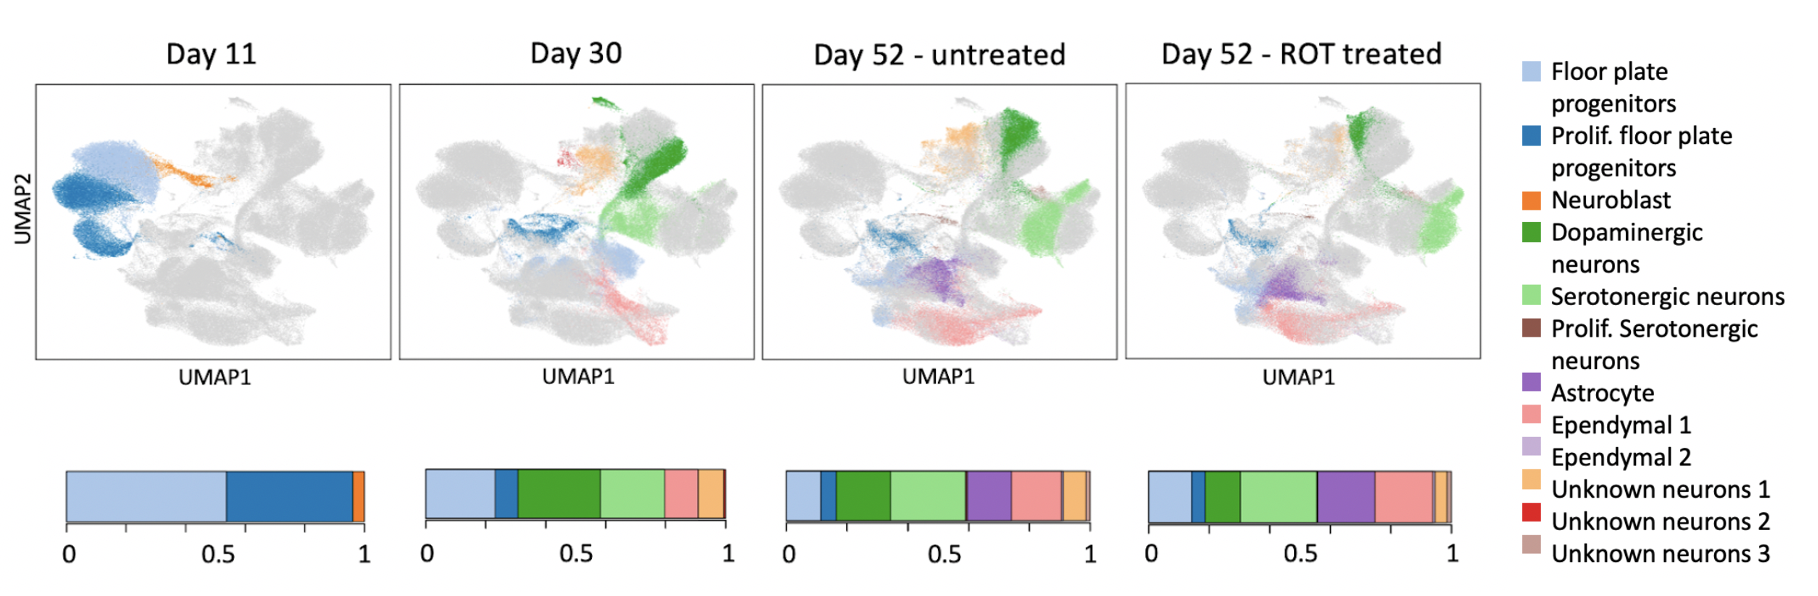
\includegraphics[width=16cm]{Chapter5/Fig/neuroseq_overview.png}
\caption[Overview of study]{\textbf{Overview of study}.\\
Top: UMAP plot of all 1,027,401 cells assayed, coloured by annotated cell type identity. Cells that were not collected at a given condition (time point, stimulus) are displayed in light grey. Prolif: Proliferating. 
Bottom: Barplot showing, for each condition, the fraction of cells assigned to each cell type.}
\label{fig:neuroseq_overview}
\end{figure}

\newpage

\section{Line-to-line variation in differentiation efficiency}

Given the great diversity in terms of cell types generated by this protocol, we investigated whether this variation may be driven by variation in differentiation outcome between different iPSC lines. 
Indeed, several studies have observed high variability in the outcome of iPSC differentiation protocols \cite{d2019association, volpato2018reproducibility}, yet the biological basis for this remains largely obscure, which hinders efforts to rationally select cell lines for specific applications. 

Here, we found substantial variation in the proportions of different cell types produced by different iPSC cell lines at each time point. 
For example, the proportion of day 52 cells assigned to DA neurons ranged from 1\% to 100\% from line to line. 

\begin{figure}[h]
\centering
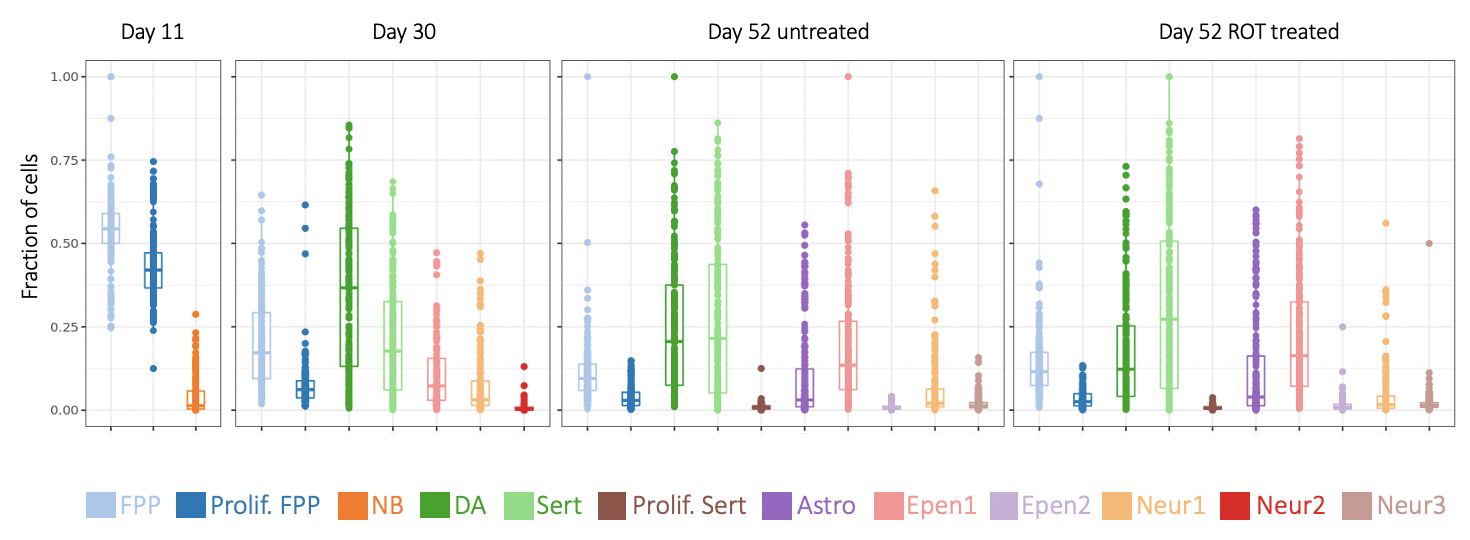
\includegraphics[width=15cm]{Chapter5/Fig/neuroseq_line_celltype.png}
\caption[Cell type fractions across lines]{\textbf{Cell type fractions across lines}.\\
Box plot showing, for each cell type, the proportions of that cell type across cell lines at day 11, day 30, untreated day 52, rotenone treated day 52. 
Each point indicates a different cell line.}
\label{fig:neuroseq_line_variation}
\end{figure}

Looking at the cell type fractions per cell line and pool, across time point we can start to observe a bimodality where roughly 2/3 of lines mostly make DA and Sert at day 30 and day 52, whilst the other 1/3 makes very few midbrain neurons but many Ependymal cells and astrocyte-like cells instead.

When we perform principal component analysis of such cell type fractions matrix, we identified the proportion of midbrain neurons (DA and Sert) on day 52 as the largest axis of variation (PC1, 47\% variance). 

\begin{figure}[h]
\centering
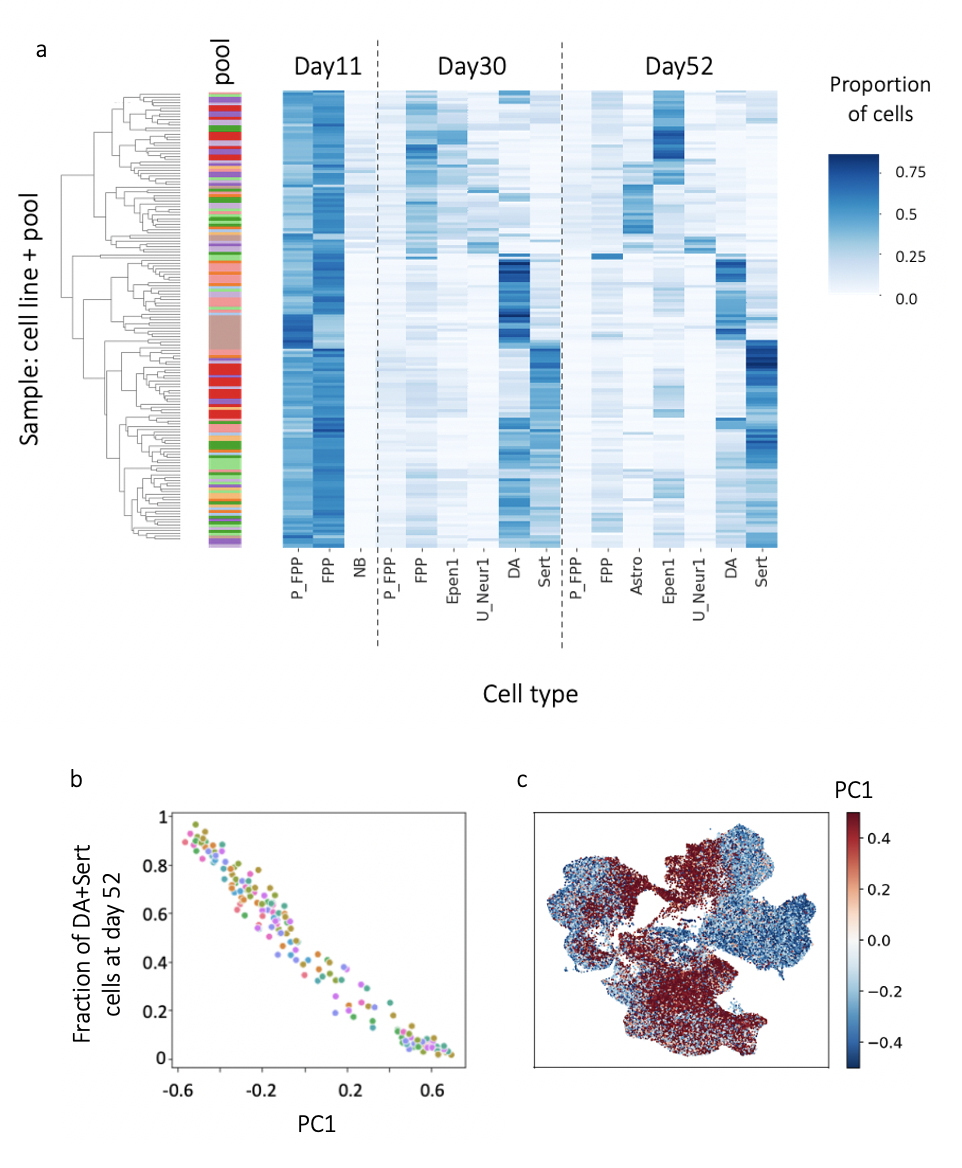
\includegraphics[width=15.5cm]{Chapter5/Fig/neuroseq_define_diff_efficiency.png}
\caption[Definition of differentiation efficiency]{\textbf{Distribution of cell proportion at day 52 and the definition of differentiation efficiency}.\\
Cell proportions were generated for each cell type and time point for all combinations of cell lines and pools with at least 10 cells at all time points (10 pools). 
(a) Heatmap of the resulting cell proportion matrix. 
Pools are shown in the first bar and the colours indicate in which of the 10 pools each line was differentiated. 
Rows (i.e. cell line, pool combinations) were hierarchically clustered according to Euclidean distance. 
(b) Comparison of the first principal component (PC1) to the sum of fractions of dopaminergic and serotonergic neurons present on day 52.}
\label{fig:neuroseq_diff_efficiency}
\end{figure}

Since DA and Sert cells are derived from similar progenitor populations \textit{in vivo}, it is not surprising that both populations are observed in our differentiation experiment \cite{ye1998fgf}. 
This motivated us to estimate a `differentiation efficiency' for each iPSC line, defined as the sum of the proportions of DA and Sert cells produced on day 52.

We assessed the reproducibility of this measure of differentiation efficiency using data from 35 lines that were differentiated twice, in two different pools. 
Importantly, we found that iPSC line differentiation efficiency defined in this way was highly reproducible between different pools (Pearson R=0.75; p value=$2x10^{-6}$).

\begin{figure}[h]
\centering
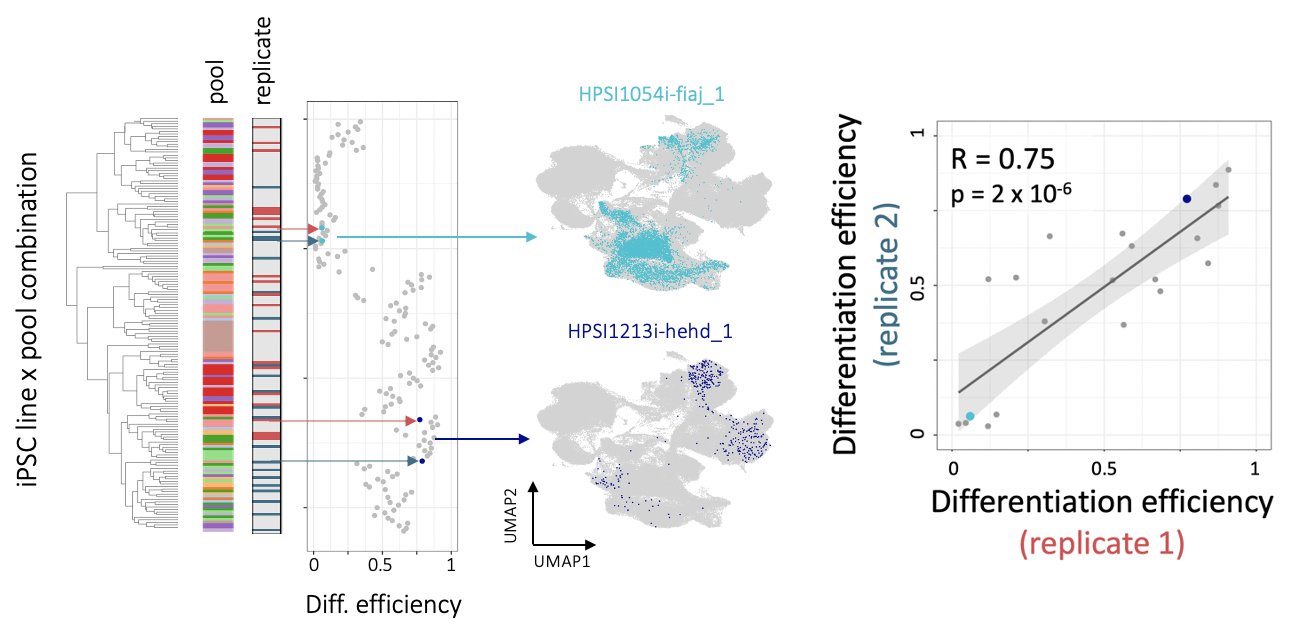
\includegraphics[width=15cm]{Chapter5/Fig/neuroseq_diff_eff_replication.png}
\caption[Reproducible differentiation efficiency]{\textbf{Reproducible variation in differentiation trajectories}.\\
Hierarchical clustering of (cell line,pool) combinations by differentiation efficiency. 
Pools are shown in the first bar and the colours indicate in which of 10 pools (for which we had data at all time points, used to define differentiation efficiency) each line was differentiated. Differentiation replicates, where the same line was present in 2 pools, are shown in the second bar (replicate 1 in red and replicate 2 in blue).
UMAPs, highlighting the distributions of cells on day 52 for two selected cell lines with low and high differentiation efficiencies respectively (HPSI0514i-fiaj\_1, in seagreen and HPSI1213i-hehd\_1, in dark blue) (right).
Scatter plot showing estimated differentiation efficiency between differentiation replicates (i.e. cell lines differentiated in two different pools, n=35). 
Highlighted are the two cell lines from (b).}
\label{fig:neuroseq_diff_eff_replication}
\end{figure}

\subsection{Organoids}
Given the robustness of these results, we wondered if they were generalisable to other neuronal differentiation approaches. 
We therefore differentiated a pool of 18 lines (pool 4) into cerebral organoids for 113 days (as previously described, \cite{lancaster2017guided}) and profiled the resulting cell populations using scRNA-seq (11,445 cells). 
The same steps of dimensionality reduction, batch correction and clustering applied to the midbrain dataset were applied to the cerebral organoid data. 
This identified eight clusters that were mapped to different cell types (neural cells, intermediate progenitor cells, radial glial progenitor cells, satellite cells, mesenchymal cells, myotube and Wnt and PAX7 positive cells) using 24
marker genes (Fig. \ref{fig:neuroseq_organoids}).
Remarkably, we found that the proportion of brain cell types (all neural, glial, and neural progenitor cells) produced by each line in the cerebral organoids was strongly correlated with differentiation efficiency as estimated from the dopaminergic differentiation (R=0.94; p value=$2x10^{-5}$; n=12). 
Taken together, these results strongly suggest that variation in iPSC neural differentiation efficiencies arise primarily due to cell-intrinsic factors. 
Furthermore, the consistency of differentiation efficiency suggests these properties extend to neuronal differentiation more generally.

\begin{figure}[htbp]
\centering
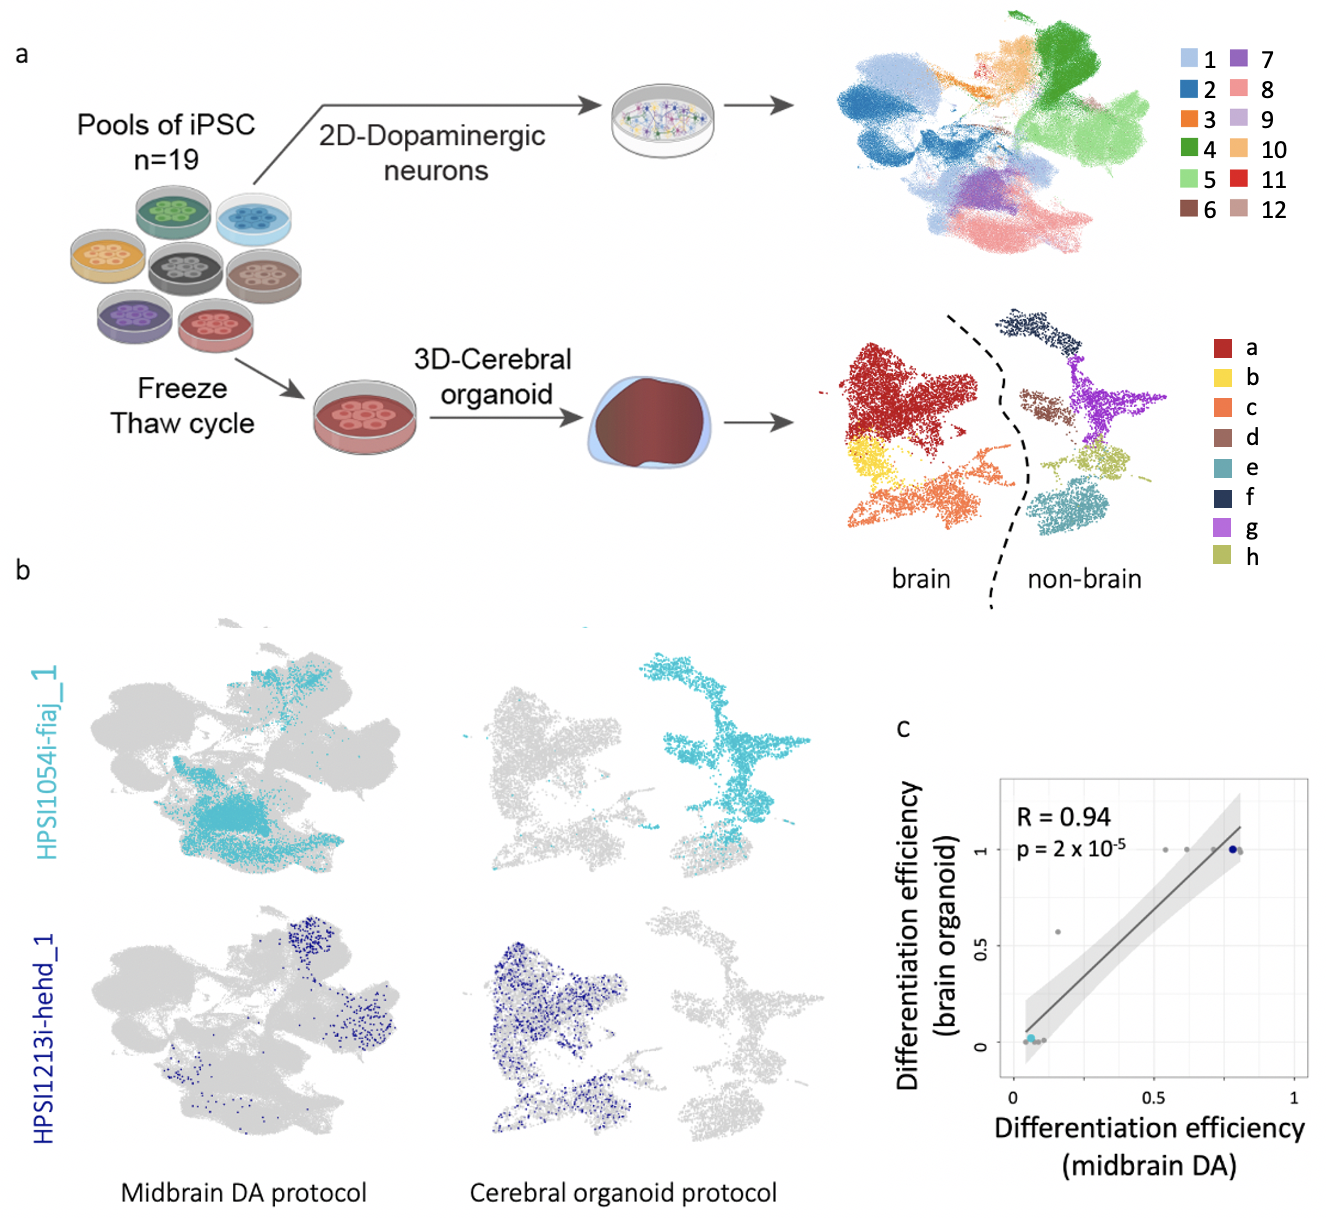
\includegraphics[width=14cm]{Chapter5/Fig/neuroseq_organoids.png}
\caption[Differentiation efficiency in cerebral organoids]{\textbf{Differentiation efficiency in cerebral organoids}.\\
(a) Experimental workflow for scRNA-seq analysis of iPSC-derived cerebral organoids using one pool consisting of 18 cell lines, profiled using scRNA-seq after 113 days of differentiation.
Add cell type legend. 
(b) UMAPs of two representative cell lines making non-brain and brain cell types in the organoid study. 
(c) Scatter plot of differentiation efficiency as measured using midbrain dopaminergic neuronal differentiation (x-axis) versus differentiation efficiency as measured in organoid differentiation (y-axis) for a subset of 12 iPS cell lines in common. 
Highlighted are the two cell lines from (b).}
\label{fig:neuroseq_organoids}
\end{figure}

\newpage

\section{iPSC expression can predict differentiation efficiency}

Motivated by the reproducibility of differentiation outcomes across multiple independent pools, we set out to explore possible predictors.
Indeed if we could find characteristics that we could measure in iPSCs that would predict in particular a bad outcome that could become a very useful tool to select lines to differentiate in future experiments.\\

We began by testing for associations between differentiation efficiency and other experimental and biological factors.
Those included cell line passage number (p=0.77), donor sex (p=0.008), chromosome X activation status (p=0.01), and PluriTest scores \cite{muller2011bioinformatic} (p=0.01). \\ % add details

Next, we assessed whether differentiation efficiency was associated with particular patterns of gene expression in undifferentiated iPSCs. 
Using data from independent bulk RNA-seq data available for a subset of 184 iPSC lines included in this study \cite{kilpinen2017common, bonder2019systematic} we identified significant associations with differentiation efficiency for 2,045 genes (983 positive and 1,062 negative associations; F-test, FDR < 5\%). 

\begin{figure}[h]
\centering
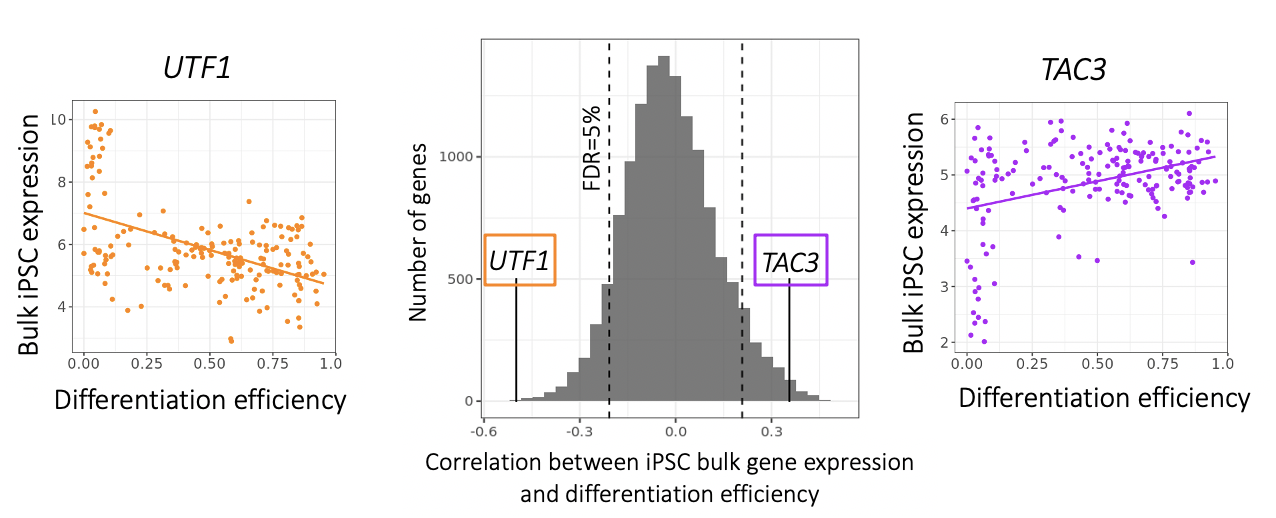
\includegraphics[width=16cm]{Chapter5/Fig/neuroseq_ips_bulk_expr_correlations.png}
\caption[iPS expression signature of differentiation efficiency]{\textbf{A gene expression signature in iPSCs is associated with differentiation efficiency}.\\
Histogram of Pearson correlation coefficients between variation in gene expression of individual genes (from bulk RNA-seq \cite{bonder2019systematic}) and differentiation efficiency. 
Two representative genes (\textit{UTF1, TAC3}) are highlighted. 
\textit{UTF1} is an example of a genes whose gene expression in iPSC (based on bulk RNA-seq) is negatively correlated with differentiation efficiency (R=-0.5, p value = = 3.5$x10^{-13}$ ), whereas \textit{TAC3} is positively correlated (R=0.38, p value = 9.8$x10^{-8}$).}
\label{fig:neuroseq_ips_expression_signature}
\end{figure}

\subsection{A predictor of (poor) differentiation using iPSC gene expression}

Next, we used the genome-wide gene expression signature in undifferentiated iPSCs to build a model to predict poor differentiation outcomes, where we defined poor differentiation as a binary outcome (differentiation efficiency < 0.2).
We used a logistic regression and obtained 100\% precision at 35\% recall as assessed by cross-validation. 
This result was robust to alternative thresholds for defining poor differentiation outcomes. 

\begin{figure}[h]
\centering
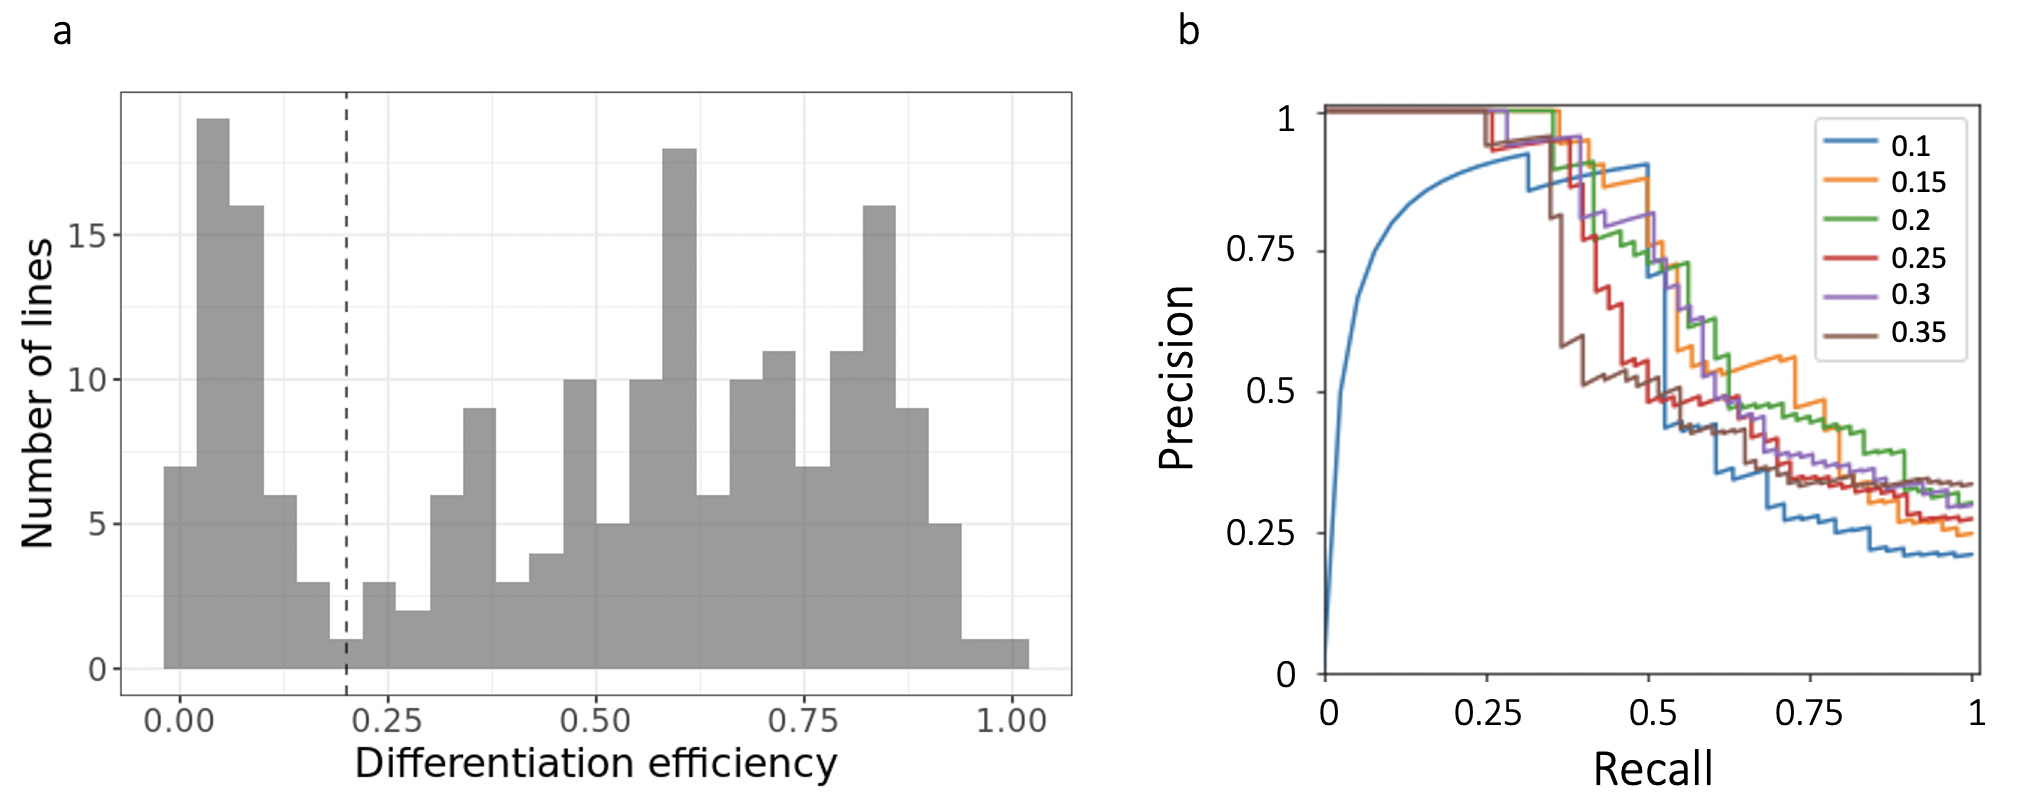
\includegraphics[width=15.5cm]{Chapter5/Fig/neuroseq_diff_eff_predict.png}
\caption[Predicting differentiation failure from iPSC gene expression]{\textbf{Predicting differentiation failure from iPSC gene expression}.\\
(a) Histogram of differentiation efficiencies across cell lines. 
The threshold chosen to define differentiation success or failure (i.e. differentiation efficiency=0.2) is shown by the dashed line, separating the two modes of the distribution. 
(b) Precision-recall curves for a logistic regression model predicting differentiation failure from iPSC gene expression data2 using a range of thresholds between 0.1 and 0.35 to define differentiation failure. 
Results are presented from leave-one-out cross validation.}
\label{fig:neuroseq_diff_eff_predictor}
\end{figure}

We then used this model to generate predicted scores for all 812 HipSci lines for which bulk RNA-seq data was available.
This analysis indicated that a substantial fraction of lines in the HipSci resource (26\%) were predicted to produce < 20\% neuronal cells under the differentiation conditions we tested.
Furthermore, we tested whether the same experimental and biological factors previously associated with differentiation efficiency replicated in this larger sample and found consistent results.
Finally, we also observed substantial variation in predicted outcomes of different lines from the same donor, suggesting that donor genetic background is unlikely to play a role in driving differentiation biases.

\subsection{A subpopulation of iPSCs is associated with poor differentiation}

Next, since iPSC cultures are heterogeneous, we hypothesised that the identified predictive gene signatures might arise from varying proportions of an iPSC subpopulation. 
To test this hypothesis, we re-analysed scRNA-seq data from 112 iPSC lines that were assayed previously under iPSC culture conditions similar to those used here 2 
\cite{cuomo2020single}, 45 of which were also included in this study). 
We identified 5 clusters, all but one of which expressed similarly high levels of core pluripotency markers (\textit{NANOG, SOX2, POU5F1}). 
We found that genes whose expression predicted poor differentiation (e.g \textit{UTF1}) were highly enriched in one of those clusters (cluster 2), while genes whose expression were predictive of successful differentiation (\textit{TAC3}), were downregulated in cluster 2 relative to the remaining iPSC clusters. 
In comparison, other cell clusters did not show such equivalent enrichment in differentiation marker genes.\\

As a direct confirmation of this hypothesis, we also tested for and confirmed an association between the fraction of cells in cluster 2 and differentiation efficiency for each cell line (Pearson R = -0.76, p value =$2.05x10^{-9}$). 

\begin{figure}[htbp]
\centering
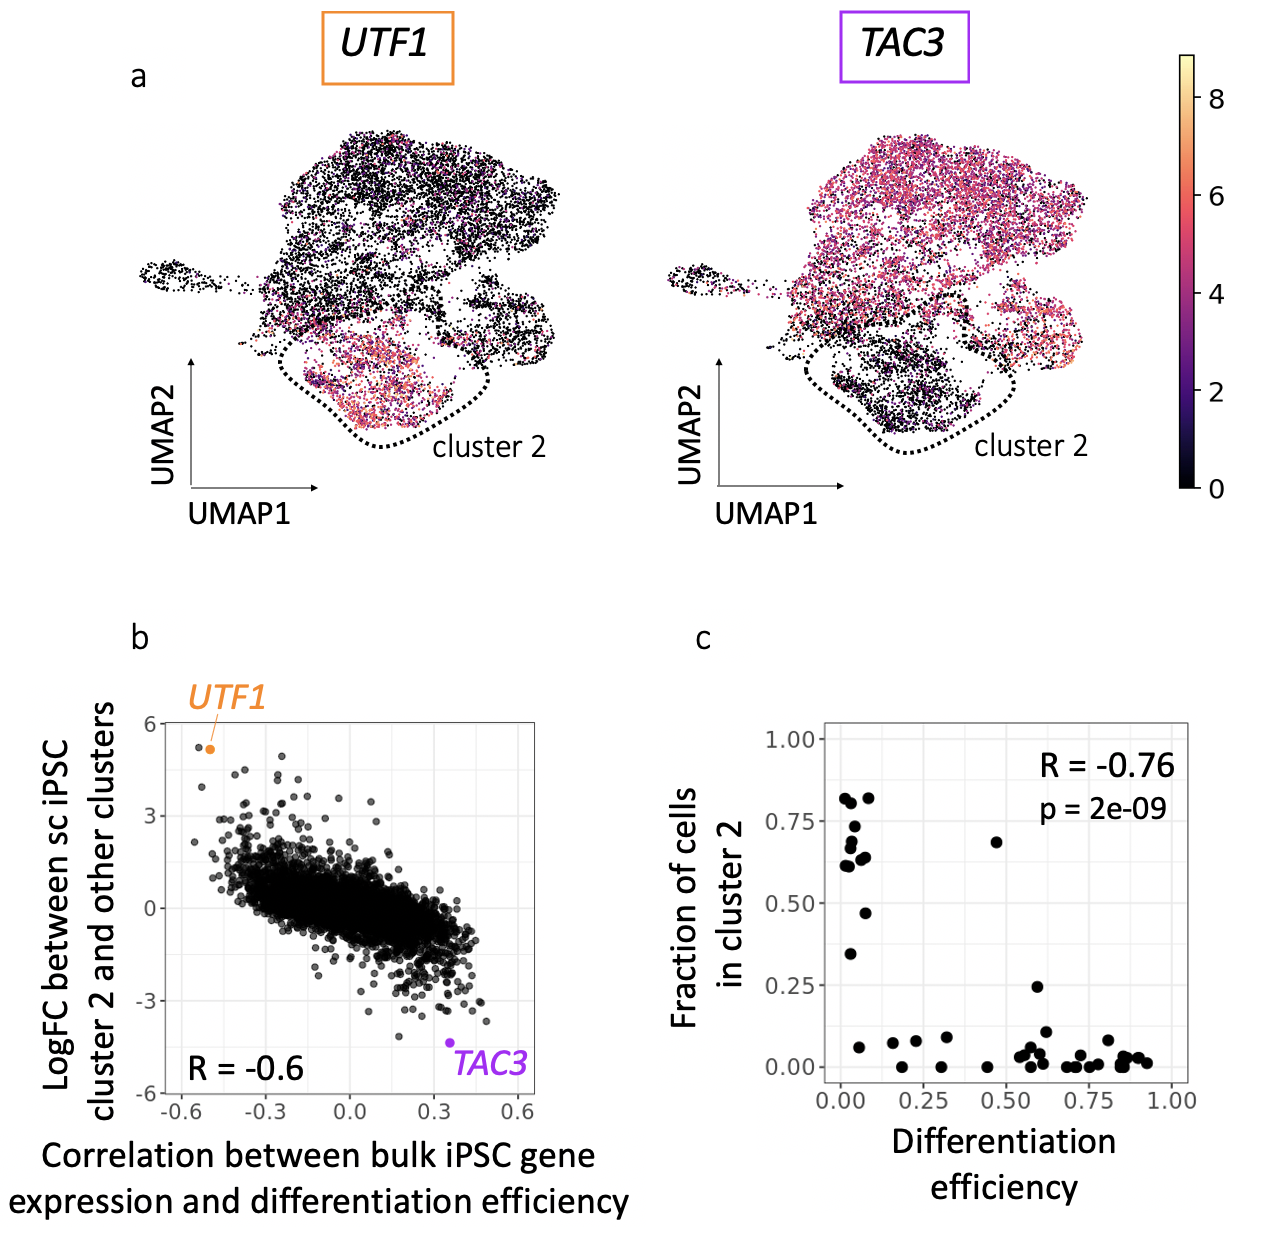
\includegraphics[width=14cm]{Chapter5/Fig/neuroseq_ips_sc_genes.png}
\caption[An iPSC subpopulation is linked to poor differentiation]{\textbf{A subpopulation of iPSCs is associated with poor differentiation}.\\
(a) UMAPs of single-cell RNA-seq profiles in iPSCs from 112 donors \cite{cuomo2020single}.
Colours denote the expression level of the two example genes from Fig. \ref{fig:neuroseq_ips_expression_signature}: \textit{UTF1} and \textit{TAC3}. 
Cluster 2 is shown by the dashed lines. 
(b) Comparison of marker gene association results with expression markers of the cluster 2. For each gene, the Pearson correlation coefficient of association between the gene and differentiation efficiency (x-axis; iPSC gene expression assessed using bulk RNA-seq, as in Fig. \ref{fig:neuroseq_ips_expression_signature}) is compared to its log fold change between cluster 2 and the other clusters (y-axis, scRNA-seq).
(\textit{UTF1, TAC3}) are highlighted. 
(c) Scatterplot between the proportion of cells assigned to cluster 2 (y-axis) and differentiation efficiency (x-axis) across 45 cell lines which were included in both sets of experiments. 
Where multiple measurements were available for a given cell line, these were averaged.}
\label{fig:neuroseq_ips_sc_genes}
\end{figure}

We used additional data from \cite{cuomo2020single} to assess the consistency of the fraction of cluster 2 cells across replication experiments, finding high concordance (Pearson R=0.9; n=23).
Using the known relationship between iPSC bulk RNA-seq and the proportion of cluster 2 cells, we predicted this proportion for 182 cell lines included in our differentiation experiments, and confirmed the negative correlation with differentiation efficiency (Pearson R = -0.49; p value = $3x10^{-12}$). 
Finally, we also analysed an additional scRNA-seq dataset from iPSCs derived from Lymphoblastoid Cell Lines (LCLs) \cite{sarkar2019discovery}. 
Using our single cell analysis pipeline, we also identified a cluster of cells with a concordant expression profile to cluster 2. 
Taken together, these results provide further evidence that a subpopulation of iPS cells with poor differentiation capability is consistently detected across different human iPSCs banks, and that this bias can be robustly predicted using expression markers at the iPSC stage. 
Importantly, despite the variability in differentiation efficiency, our single-cell sequencing approach enabled us to examine multiple disease-relevant cell populations for many cell lines. Correlating changes in gene expression with common genetic variants associated with various traits in GWAS could provide insights into disease mechanisms.

\newpage

\section{eQTL mapping in neuronal cell types}

Next, we mapped eQTL in order to understand how individual-to-individual genetic variation influenced gene expression across these cell types during differentiation and in response to stimulation.

Specifically, we mapped \textit{cis} eQTL in each of the well represented\footnote{top 4
cell type per condition with at least 20\% cells} `cell type'-`condition' contexts defined above.
We mapped eQTL independently for each of the 14 distinct cell populations shown in Table \ref{tab:eqtl_maps}. 

\begin{table}[h]
    \centering
    \begin{tabular}{c|c c c c c c}
    &         FPP & P\_FPP & DA & Sert & Epen1 & Astro \\
    \hline
    Day 11  &  \checkmark & \checkmark   \\
    Day 30  & \checkmark & & \checkmark & \checkmark & \checkmark  \\
    Day 52 - untreated & & & \checkmark & \checkmark & \checkmark & \checkmark \\
    Day 52 - ROT treated & & & \checkmark & \checkmark & \checkmark & \checkmark \\
    \end{tabular}
    \caption{eQTL maps}
    \label{tab:eqtl_maps}
\end{table}

eQTL were mapped by calculating aggregate expression levels for each donor, considering common gene-proximal variants (MAF > 0.05, plus or minus 250 kb around genes). 
Variability in differentiation efficiency between lines\footnote{i.e. some lines made mostly neuronal cell types and barely any non-neuronal, thus expression estimates for those lines in non-neuronal cell types will be less accurate because estimated using very few cells, and viceversa for lines that mostly made non-neurons, and very few donors.} resulted in substantial differences in the number of cells collected for each donor, affecting accuracy of the estimates of aggregated expression. 
To account for this source of noise, we adapted commonly used eQTL mapping strategies \cite{cuomo2020single} based on \glspl{lmm} by incorporating an additional variance component into the model:

\begin{equation}
    \mathbf{y} = \mathbf{W}\boldsymbol{\alpha} + \mathbf{g}\beta + \tilde{\mathbf{u}} + \boldsymbol{\psi}, 
\end{equation}

where $\tilde{\mathbf{u}} \sim N(\mathbf{0}, diag(\frac{1}{n_i}))$, where $n_i$ is the number of cells for each individual i.\\

Because we are not accounting for population structure in the model, we have to rely on samples being unrelated, and cannot consider multiple observations for the same lines (e.g. across pools). 
As a consequence, expression was aggregated at the cell line (and therefore donor) level, averaged across two pools for the lines present in more than one pool.

This approach greatly increased the power to map eQTL, resulting in a total of 4,087 genes with at least one eQTL in any of the contexts (hereafter `eGene', FDR < 5\%).

Our approach also improved power compared to other model tried to address reviewers..

\subsection{Comparison of eQTL across cell types and conditions}

The largest number of eQTL were detected in progenitor cell populations, likely reflecting increased detection power due to the larger number of well-represented donors (> 100 cells per donor; Methods, Supplementary Fig. 8). 
Notably, the cumulative number of genes with an eQTL in each cell type increased substantially when considering cells further progressed along the differentiation axis, as well as upon stimulation (Fig. 4a). 


\begin{figure}[h]
\centering
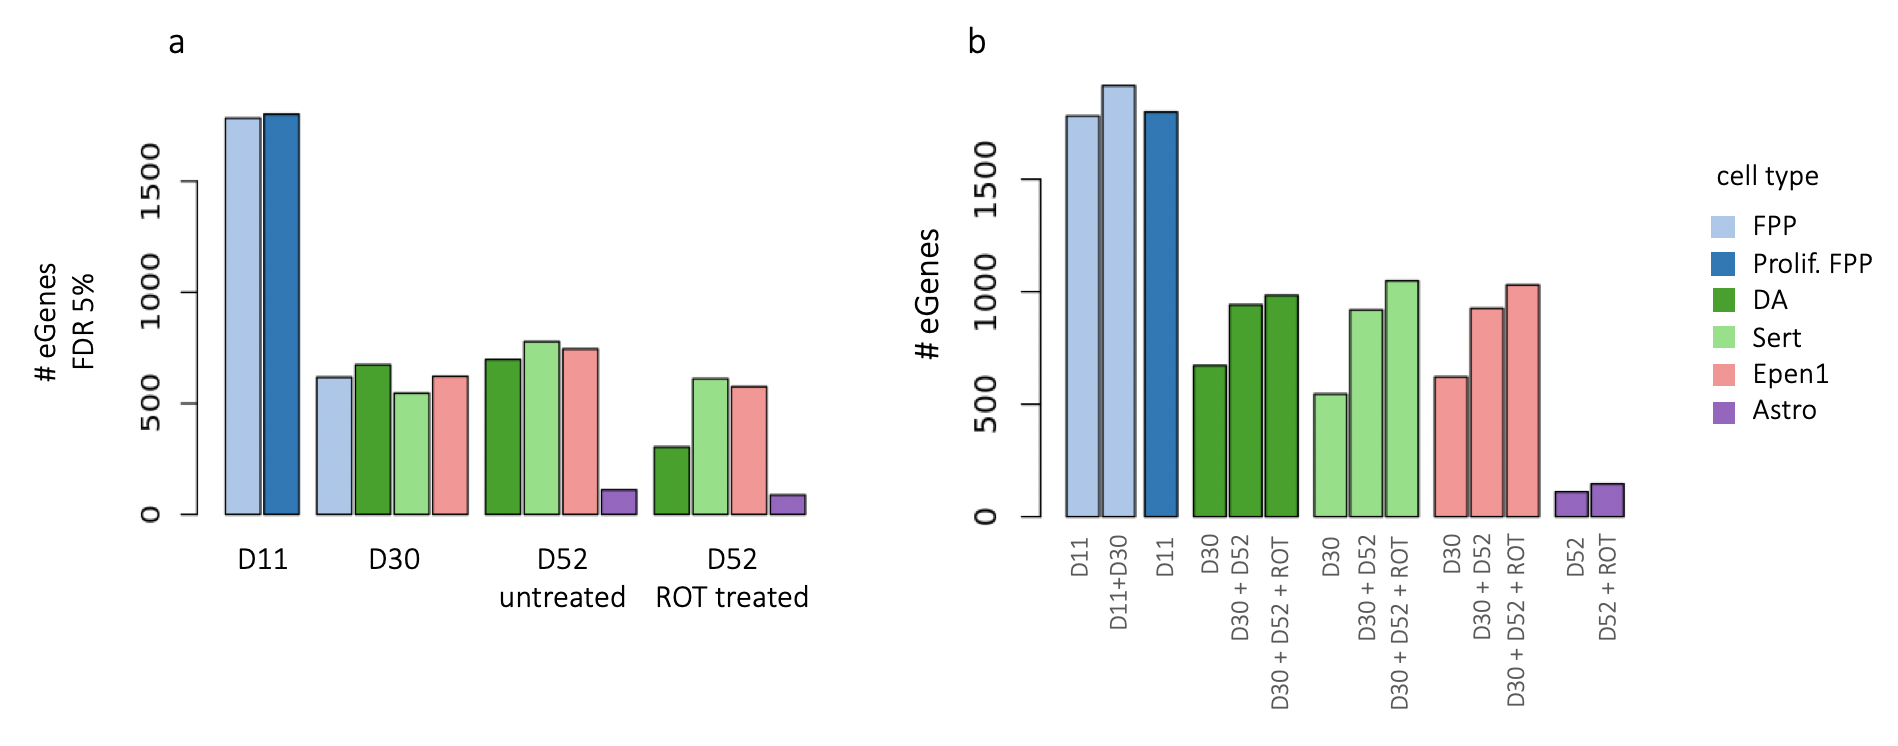
\includegraphics[width=16cm]{Chapter5/Fig/neuroseq_eqtl.png}
\caption[Mapping eQTL across neuronal cell types]{\textbf{Mapping \textit{cis} eQTL in distinct cell contexts (`cell types'-`conditions') across midbrain differentiation.}.\\
(a)Number of genes with at least one eQTL (eGenes) for each cell type and condition.
(b)Cumulative number of eGenes for each cell type and condition (D11 = Day 11; D30 = Day 30; D52 = Day 52; ROT = Rotenone stimulation).}
\label{fig:neuroseq_eqtl}
\end{figure}

For example, in DA cells, eQTL mapping in matured cells (day 52) identified an additional set of 270 egenes compared to day 30 cells.\\

An example of a timepoint-specific eGene is \textit{HSPB1}, for which SNP rs6465098 is an eQTL in day 52 cells, but not day 30 (Fig. 4b). 
\textit{HSPB1} encodes a heat shock protein that plays a key role in neuronal differentiation \cite{miller2018heat} and for which changes in gene expression have been observed in neurons after ischemia \cite{bartelt2016hspb5} and associated with toxic protein accumulation in Alzheimer disease \cite{shimura2004binding, wilhelmus2006small}.\\

Similarly, we detected 196 additional eGenes with a rotenone-specific effect in DA and Sert neurons. 
As an example, rs12597281 is an eQTL for \textit{ACSF3} in rotenone stimulated serotonergic neurons at day 52, but not in unstimulated cells (Fig. 4b). 
\textit{ACSF3} encodes an acyl-CoA synthetase localized in the mitochondria and for which inherited mutations have been associated with a metabolic disorder, combined malonic and methylmalonic aciduria (CMAMMA), where patients exhibits a wide range of neurological symptoms including memory problems, psychiatric problems and/or cognitive decline \cite{tucci2020brain}.\\

These examples highlight how changes in the expression of genes known to be associated with human disease can be transient and specific to a cell type and state. More importantly, this data shows how our experimental design brings an extra level of resolution to understand the disease mechanisms that were previously inaccessible from primary tissues and open up new experimental avenues.

\subsection{Comparison of eQTL from our study and \textit{in vivo} maps}


To test how our eGene discovery relates to previous studies, we compared the number of eGenes identified in this study with bulk eQTL maps from \textit{in vivo} tissues from the GTEx consortium \cite{gtex2017genetic}. 
To aid the comparability between bulk and single-cell eQTL maps,
we aggregated eQTL across cell types and found that the number of discovered eGenes
was similar to that expected in a primary tissue of the same sample size (Fig. 4c). However, when focusing on individual cell populations, we observed fewer “cell type”-“condition” eQTL than detected in GTEx tissues of similar sample size, likely due to the decreased representation of donor cells.\\

A key question of eQTL maps from in vitro iPS-based models is how closely these resemble eQTL maps from primary tissues that differ in cell composition. 
To explore this, we tested the extent to which regulatory variants were shared between eQTL maps in three resources: 1) the current study, 2) GTEx brain tissues (n=13 tissues), and 3) bulk and single-cell RNA-seq profiles of HipSci iPS cell lines \cite{bonder2019systematic, cuomo2020single}, as measured by genome-wide consistency of eQTL effect sizes (using MASHR 42 \cite{urbut2019flexible}). 
We found that as iPSCs were differentiated to increasingly mature neuronal cell types, the extent of eQTL sharing consistently increased (Fig. 4d). 
This provides additional confidence that eQTL discovered in iPS-derived neuronal
populations mimic \textit{in vivo} eQTL maps. 
Consistent with the trend of increased eQTL sharing, we also observed that the fraction of eQTL that are not represented in GTEx brain tissues decreases as the cells become more mature (Supplementary Fig. 9a). 
Interestingly, while iPS-derived eQTL maps mimic \textit{in vivo} GTEx Brain eQTL maps, we also identified 2,203 eQTL that could not be detected in GTEx brain tissues (q-value > 0.05 in any of 13 tissues), demonstrating the utility of iPSC and scRNA analysis to discover regulatory changes in disease associated genes.\\
%%

% In Chapter 4 we have focused on reproducing standard `mean-level' expression level eQTL mapping using scRNA-seq, where the phenotype of interest is expression abundance within a homogeneous population of cells.
% We can call such efforts `pseudo-bulk' approaches, where we are essentially replicating bulk-like expression values and performing the eQTL test adapting approaches used for traditional eQTL mapping using bulk RNA-seq. 
% In the applications we and others have described \cite{van2018single,cuomo2020single}, the value of using scRNA-seq lies in the fact that we are able to, within a single experiment, unbiasedly define and assess multiple different cell types, whilst retaining a single cell resolution.\\

\section{Colocalisation of eQTL with disease risk variants}

The identified cell-type specific eQTL maps across different differentiation contexts provide a unique opportunity to understand human disease traits and their genetic risk factors identified by genome-wide association studies (GWAS). 
To systematically test for such colocalisation events, we applied COLOC \cite{giambartolomei2014bayesian} to the summary statistics from 25 n eurological traits, eQTL discovered in our study, as well as eQTL obtained from GTEx (Supplementary Table 8,9).\\

In total, we identified 1,052 eQTL in our study with evidence of colocalisation with at least one disease trait, 485 of which were found only in our data set. 
This corresponds to an additional ~10\% of colocalisation events of GWAS variants compared to eQTL across all GTEx tissues (5,028 across 48 tissues, Fig. 5b). 
Notably, 298 (61\%) of the colocalisations in our data were associated with eQTL detected in later differentiation stages (day 52) or upon stimulation (day 52 ROT, Supplementary Fig. 9b ).\\

Among the most interesting colocalisation events was an eQTL for \textit{SFXN5}, a mitochondrial amino-acid transporter, which was specific to the rotenone-stimulated serotonergic neurons at day 52, and which co-localized with a Schizophrenia hit (PP4 = 0.76, Fig. 5c). 
Exposure to rotenone is known to induce oxidative stress by inhibiting the mitochondrial respiratory chain complex I \cite{palmer1968studies, betarbet2000chronic}. 
We therefore speculate that the specific genetic signal observed for the mitochondrial gene \textit{SFXN5} in serotonergic neurons is a possible factor modulating environmental stress response.\\

Another example that colocalized with a Schizophrenia GWAS variant was an eQTL for
\textit{FGFR1}, detected both in proliferating and non proliferating floor plate progenitors at day 11 (PP4 = 0.93 and 0.88 respectively, Fig 5d) . 
Previous studies have shown that nuclear \textit{FGFR1} plays a key role in regulating neural stem cell proliferation and central nervous system development, in part, by binding to the promoters of genes that control the transition from proliferation to cell differentiation \cite{ma2009molecular}. 
Additionally, it was shown that altered \textit{FGFR1} signaling was linked to the progression of the cortical malformation observed in schizophrenia \cite{stachowiak2017cerebral}.\\

These examples suggest that a combination of genetic and environmental factors during an early developmental stage might contribute to schizophrenia pathology and illustrate how these data represent a valuable resource to understand the molecular basis of complex neurological disease.

\newpage

\section{Discussion}

% disease relevance

% protocol efficiency

% cell type composition - joint model\\

Characterising the function of human trait-associated genetic variation requires large scale studies performed in disease-relevant cell types and states. 
Here, we demonstrate how human iPSCs can be efficiently profiled at scale throughout a long-term differentiation to a midbrain cell fate. 
We uncover a highly reproducible, cell-intrinsic neuronal differentiation bias and show how this bias can be robustly predicted using simple gene expression profiling in the pluripotent cell state. 
This result sets the stage for the optimized design of future large scale iPSC experiments, where cell lines can be rationally selected a priori without the need for laborious testing of differentiation capacity. 
Importantly, our analysis also identified several hundred trait-associated genetic changes in gene expression that have not been previously identified. 
Overall, our study demonstrates the utility of pooled iPSC differentiation and single-cell analysis for revealing the function of disease-associated genetic variation in otherwise inaccessible cell states.\\

Despite a modest sample size, our study reveals a disproportionately large number of novel disease-eQTL colocalisations compared with GTEx tissues of equivalent sample size. 
For example, the number of novel disease-eQTL colocalisations added by GTEx liver or cerebellar hemisphere (n=208, 215 respectively) are 80 and 107, respectively, compared to 485 in this study. 
A simple explanation for this result is that our experiment profiled expression states that are hard to capture using post-mortem tissue, including timepoints during neuronal differentiation and rotenone exposure. 
Additionally, we detected many eQTL that were specific to individual cell types, enabled by the single-cell resolution of our study.
These signals, while present, are challenging to detect in bulk tissue because the relevant cell types are often rare. 
Taken together, these results suggest that many “missing”, disease-relevant eQTL likely remain to be discovered using single cell sequencing of both primary tissue and \textit{in vitro} cell models.\\

A second implication of our study is that, despite growth competition between cell lines, multiplexing experiments retain sufficient cells per donor to perform robust genetic analysis, even following extended periods in culture (Supplementary Fig. 8, Supplementary Table 2). 
Although cell lines were pooled at similar numbers, we observed extensive variation throughout our experiment in the numbers of cells produced by different lines. 
For example, 50\% of the cells we sequenced were produced by only 12\% of lines.
Future technical improvements, such as more precise matching of growth rates of cell lines within pools, or line selection based on predicted differentiation capacity using markers in the iPS state may further increase the utility of multiplexed iPSC differentiation.

The “quality” of human iPSCs has previously been carefully examined using both genetic and functional genomic data \cite{muller2011bioinformatic, international2018assessment, tsankov2015qpcr, bock2011reference}. 
Despite these efforts, differentiation bias among cell lines has been widely appreciated but poorly understood. 
The underlying mechanisms have been hypothesised to involve epigenetic factors, environmental factors such as culture conditions, or changes acquired by cells over time in culture, or cell type of origin. 
To the best of our knowledge, the work presented here is the first to systematically survey differentiation biases at the scale of an entire cell bank. 
To address this question, we leveraged the large number of cells in the HipSci bank and the detailed phenotyping of each of these lines. 
We excluded the cell type of origin hypothesis \cite{hu2016effects} in this instance since all HipSci lines were skin-derived.
We also observed relatively weak relationships between differentiation efficiency and other biological factors, such as X chromosome inactivation status, which has been described as relevant for other differentiation lineages \cite{cuomo2020single}.
Instead, we found that variability in differentiation outcomes can be largely explained by cell-intrinsic factors that are maintained over multiple freeze/thaw cycles. 
When we tested if these factors were due to the genetic variant inherited from the donor (\cite{kajiwara2012donor}), we found that a strong donor component was unlikely due to the poor
correspondence in predicted differentiation outcomes between lines derived from the same individual ( Supplementary Fig. 5c,d,e ). 
Additionally, we did not detect significant effects in a genome-wide association analysis with predicted differentiation outcomes (p>5x10 -8 , n=540, MAF=0.05). 
Given these results, we suggest the two most likely candidates for future investigation are somatic genetic changes or persistent changes to cell line epigenomes that occur early in cellular reprogramming.\\

In particular, our analysis indicates that the reduced production of neurons was best
correlated with increased abundance of a specific subpopulation (cluster 2) of pluripotent cells that express the transcription factor UTF1 and other genes at elevated levels.
Counter-intuitively, the proportion of cells in this subpopulation was positively correlated with the proportion of neuroblast cells on day 11, but lower fractions of dopaminergic and serotonergic neurons at later stages of differentiation. One possible explanation is that cell lines that commit earlier to a neuronal fate disproportionately lose neurons upon passaging at Day 20. 
Alternatively, cluster 2 may preferentially give rise to radial glial cells that more readily switch to an astroglial and ependymal differentiation programme \cite{spassky2005adult}. 
In support of this hypothesis, we identified several upregulated genes in cluster 2, including \textit{SIX3}, \textit{MT1F} and \textit{PITX2}, that are thought to play a role in astrocyte and ependymal cell biogenesis \cite{lavado2011six3, michael2011up, jacquet2009foxj1} (Supplementary Table 4). 
We speculate that culture methods that reduce iPSC heterogeneity may reduce the fraction of iPSC lines that resist efficient neuronal differentiation. 
We also note that our findings do not explain all of the variance in neuronal differentiation capacity, and future studies will be required to more fully understand the biological basis of the differentiation bias we have observed here.\\

Based on molecular markers that are predictive for differentiation bias, we estimate that 16\% of iPSC lines in the HipSci resource produce few to no identifiable neuronal cell types under the conditions tested. 
While the production of neuronal cells was intrinsically limited in these cell lines, the fact that this effect was associated with particular cell lines but not with particular donors suggests that cell banks that contain multiple lines per donor can be most effectively utilised for applications involving neural differentiation by the rational selection of cell clones. 
Importantly, this a priori selection is enabled by gene expression profiling data from the pluripotent state that is easily obtainable and often already available.\\

In summary, our study clearly demonstrates how iPSC differentiation combined with single cell RNA-seq unlocks population level studies in increasingly complex, dynamic and biologically realistic cellular models. We anticipate that future uses of this model system will focus on experimental settings that are challenging or impossible with primary cells. 
These could include high resolution sampling along extended differentiation times to more complex differentiation trajectories, such as cell organoids, or involve large panels of disease relevant-stimuli and drug exposures. 
Collectively, our study will guide future efforts to understand the common genetic basis of neurological disorders, and facilitate the development of iPSC-based approaches for modelling and treating these diseases.